\documentclass[12pt, letterpaper]{article}
% \usepackage[utf8]{inputenc} --- Since we're switching to the luatex compiler, I'm commenting this out since it will throw errors. Additionally, luatex is already UTF-8 by default.
\usepackage[T1]{fontenc}
\usepackage{lmodern}
\usepackage{textcomp}

%%%%%%%%% This preamble was copied over from my cl-freelock gh-pages branch.

% NOTE 1: lwarpmk clean to fix corrupted aux files. Corrupted aux files means no hyperlinks.
% NOTE 2: Because Biber was never ran against Manual_html, the HTML pages have broken citation links and an empty bibliography (hence: "Package biblatex Warning: Please (re)run Biber on the file: Manual_html"
% NOTE 3: lwarp relies on "patching" packages like biblatex and cleveref to translate their complex TeX commands into valid HTML. When it reports "Patching failed," it means lwarp could not successfully intercept the commands to convert them into HTML hyperlinks.
% "Package biblatex Warning: Patching footnotes failed"

\usepackage[margin=1in]{geometry}
\setlength{\marginparwidth}{2cm}
\usepackage{amsmath, amssymb}
\usepackage{csquotes}

% n.b, I had to run sudo pacman -S texlive-plaingeneric ...
% extra/texlive-plaingeneric 2026.1-1 (texlive)
% usr/share/texmf-dist/tex/latex/tracklang/tracklang.sty
% datetime2 requires tracklang.sty ...
% Verify it can be found with kpsewhich tracklang.sty
\usepackage[style=iso]{datetime2}
\usepackage[
mathjax,
ImagesDirectory=imgs,
ImagesName={lateximg-}
]{lwarp}
\usepackage[font=small]{caption}
\usepackage{tabularx}
\usepackage{booktabs}
% n.b., Because lwarp fundamentally rewrites how floating environments (like figures and tables) are handled to prevent them from actually "floating" in an HTML document, it requires the float package to be loaded after lwarp so it can properly apply its HTML specific patches over float's definitions.
\usepackage{float}
\usepackage{listings}
% lwarp actually does have special HTML patches for setspace so it must be after lwarp:
\usepackage{setspace}
\doublespacing
% n.b., after an hour of debugging, I have learned that for lwarp v0.9+ graphics and color packages must be loaded after lwarp to avoid crashing the Gin@setfile HTML patcher...
% additionally, hyperref must be loaded before biblatex, but after lwarp.
% Additionally, I later learned that html does not support nested footnotes. i.e., autocite will not be rendered with hyperlinks inside a footnote, in lwarp generated html...this explains why the hyperlinks worked in the pdf, but not in the html. Therefor, any citations made inside a footnote must use \cite, not \autocite
\usepackage{graphicx}
\graphicspath{{imgs/}}
\usepackage{xcolor}
\usepackage{tikz}
\usetikzlibrary{calc, positioning}
\usetikzlibrary{decorations.pathreplacing}
\usepackage{tcolorbox} % I'm using this as a user-facing replacement for todonotes, since lwarp explcitly supports it.
\newtcolorbox{disclaimerbox}{
	colback=yellow!10!white,
	colframe=red!75!black,
	fonttitle=\bfseries,
	title=Documentation Notice
}
% n.b., Even with the [disable] option, the todonotes package inherently loads tikz and xcolor (or color) in the background to set up its infrastructure.
\usepackage[disable]{todonotes}

\usepackage[colorlinks=true, linkcolor=blue, citecolor=blue, urlcolor=blue]{hyperref}
\usepackage[style=authoryear,backend=biber]{biblatex}
\addbibresource{references.bib}
% \usepackage{enumitem}

\widowpenalty=10000
\clubpenalty=10000
\DeclareRobustCommand{\code}[1]{%
	\begingroup
	\setlength{\fboxsep}{2pt}%
	\colorbox{gray!15}{\ttfamily\small #1}%
	\endgroup
}
\newcommand{\supcom}{%
	\textsuperscript{,}
}
\newcommand{\multicomment}[1]{}

\newcommand{\customitem}[2]{%
	\noindent\textbf{#1}\\[0.5ex]%
	#2\vspace{1ex}%
}

\makeatletter
\def\blfootnote{\xdef\@thefnmark{}\@footnotetext}
\makeatother
\lstnewenvironment{fennelcode}
{\lstset{
		language=Lisp,
		alsoletter={-,:,?,>}, % Allow standard Fennel characters in keywords
		morekeywords={
			fn, lambda, let, local, var, set, each, for, while, do,
			if, when, match, macro, import-macros, require-macros,
			quote, unquote, hashfn, length, ipairs, pairs,
			collect, icollect, accumulate, doto, ->, ->>,
			nil, true, false, pandoc, table, string, math, require
		},
		basicstyle=\ttfamily\small\linespread{1}\selectfont\raggedright,
		columns=fullflexible,
		keepspaces=true,
		upquote=true,
		keywordstyle=\color{blue}\bfseries,
		commentstyle=\color{green!60!black}\itshape,
		stringstyle=\color{red},
		breaklines=true,
		showstringspaces=false,
		aboveskip=1.5em,
		belowskip=1.5em,
		xleftmargin=0pt,
		backgroundcolor=\color{gray!10},
		frame=single,
		framerule=1.5pt,
		rulecolor=\color{black}
}}
{}

\lstnewenvironment{luacode}
{\lstset{
		language=[5.3]Lua,
		basicstyle=\ttfamily\small\linespread{1}\selectfont\raggedright,
		columns=fullflexible,
		keepspaces=true,
		upquote=true,
		keywordstyle=\color{blue}\bfseries,
		commentstyle=\color{green!60!black}\itshape,
		stringstyle=\color{red},
		breaklines=true,
		showstringspaces=false,
		aboveskip=1.5em,
		belowskip=1.5em,
		xleftmargin=0pt,
		backgroundcolor=\color{gray!10},
		frame=single,
		framerule=1.5pt,
		rulecolor=\color{black}
}}
{}

\lstnewenvironment{bashcode}
{\lstset{
		language=bash,
		alsoletter={-},
		morekeywords={
			sudo, git, apt, apt-get, pacman, echo, cd, ls, mkdir, 
			rm, mv, cp, export, source, make, cmake, ql, luarocks, lua, fennel
		},
		basicstyle=\ttfamily\small\linespread{1}\selectfont\raggedright,
		columns=fullflexible,
		keepspaces=true,
		upquote=true,
		keywordstyle=\color{blue}\bfseries,
		commentstyle=\color{green!60!black}\itshape,
		stringstyle=\color{red},
		breaklines=true,
		showstringspaces=false,
		aboveskip=1.5em,
		belowskip=1.5em,
		xleftmargin=0pt,
		backgroundcolor=\color{gray!10},
		frame=single,
		framerule=1.5pt,
		rulecolor=\color{black}
}}
{}

\newcommand{\lastedited}{%
	Last edited: \DTMnow\ UTC%
}
\date{\lastedited}
\setcounter{FileDepth}{1}
\title{fplot Manual}
\author{Andrew D. France}
\date{\lastedited}

\begin{document}
	
	\maketitle
	\tableofcontents
	\newpage
	
	\section{Welcome to the fplot Wiki!}
	
	\textbf{fplot} is a plotting library for Fennel and Lua that makes it easy to create a wide range of plots using Gnuplot. This wiki provides comprehensive documentation to help you get started making the most of its features.
	
	\begin{disclaimerbox}
		Currently, the fplot pages are just a mirror of the fplot wiki.
		Future updates will reorganize this structure to better suit a standalone manual.
		Additionally, we will add more examples of biotech related plots, such as standard curves for electrophoresis.
		Gnuplot's curve fitting in this context is usually done with the fit command, which performs non-linear least-squares curve fitting using the Marquardt-Levenberg algorithm.
		Additionally, we may include plots which are relevant to NCBI BLAST, such as distance tree/cladogram, pairwise alignment view, description table (with scores, E-values, percent identity, etc), and circos plots as they relate to flow cytometry. 
	\end{disclaimerbox} \blfootnote{Basic Local Alignment Search Tool (NCBI BLAST) is a bioinformatics program that finds regions of local similarity between biological sequences. In other words, it compares nucleotide or protein sequences to sequence databases and calculates the statistical significance of matches. \cite{ncbiblast} \cite{altschul1990blast}}
	
	\subsection*{Getting Started}
	
	If you're new to \texttt{fplot}, here are a few pages to get you up and running:
	
	\begin{itemize}
		\item \textbf{Installation:} Learn how to install \texttt{fplot} and its dependencies.
		\item \textbf{Getting Started Tutorial:} A step-by-step guide to creating your first plot.
	\end{itemize}
	
	\subsection*{Core Concepts}
	
	Understanding these two concepts is key to using \texttt{fplot} effectively:
	
	\begin{itemize}
		\item \textbf{Configuration Options:} This is where you define the overall appearance of your plot, such as its title, labels, size, and output format.
		\item \textbf{Dataset Configuration:} This is where you define the data to be plotted, along with its style, title, and other attributes.
	\end{itemize}
	
	\subsection*{Advanced Topics}
	
	Once you've mastered the basics, you can explore more advanced features:
	
	\begin{itemize}
		\item \textbf{Advanced Features:} Learn about creating multiplots, adding custom labels and arrows, and more.
		\begin{quote}
			\textbf{Macros:} A dedicated page for creating various macros
		\end{quote}
		\item \textbf{Examples:} A gallery of examples showcasing various types of plots you can create with \texttt{fplot}.
		\item \textbf{BioTech:} A gallery of examples showcasing biotech relates plots.
	\end{itemize}
	
	\subsection*{Why fplot?}
	
	\texttt{fplot} makes \texttt{gnuplot} a programmatic citizen in your Fennel and Lua projects. Instead of shelling out to separate scripts, you can define, generate, and integrate plots directly within your application's (and/or pipeline's) logic. \texttt{fplot} replaces the error-prone process of building command strings with a clean, table-based API where you describe your plot as a data structure. This makes your plotting code more readable, but more importantly, it makes your plots composable: you can build, combine, and reuse styles and datasets as regular pieces of data in your code.
	
	\subsection*{Why Fennel?}
	
	\texttt{fplot} is written in Fennel and is designed to feel most natural when used from a \texttt{.fnl} file. While it has first-class support for Lua, here are a few reasons why you might enjoy using Fennel for your plotting scripts:
	
	\begin{itemize}
		\item \textbf{Concise Syntax for Data:} Fennel's Lisp-based syntax is exceptionally clean for defining the nested tables that fplot relies on. This often results in less visual noise (fewer commas, brackets, and braces) and makes complex configurations easier to read at a glance.
		\item \textbf{Powerful Macros:} Fennel offers a true, Lisp-style macro system, allowing you to extend the language with new syntax and create powerful abstractions that are impossible in pure Lua. While not necessary for basic plotting, it opens the door for creating highly customized plotting DSLs (Domain-Specific Languages) tailored to your specific needs.
		\item \textbf{Seamless Lua Interoperability:} Fennel compiles directly to Lua. This means you lose none of Lua's performance or its rich ecosystem. You can use any Lua library (including LuaJIT) and get the best of both worlds: a powerful Lisp syntax on a fast, proven runtime.
		\item \textbf{A More Ergonomic API:} The fplot API was designed with Fennel's keywords (e.g., \texttt{:title}, \texttt{:x-label}) in mind. While perfectly usable from Lua with the \texttt{["key-name"]} syntax, the original \texttt{kebab-case} keywords feel most at home in a Fennel environment.
	\end{itemize}
	
	\noindent\rule{\textwidth}{0.4pt}
	\textbf{Resources}
	
	\noindent
	Fennel Language. (n.d.). \textit{Official documentation}. \url{https://fennel-lang.org/} \\
	Gnuplot. (n.d.). \textit{Official documentation}. \url{http://gnuplot.info/documentation.html}
	
	\newpage
	
	\section{Installation}
	
	This page guides you through installing \texttt{fplot} and its required dependencies.
	
	\subsection{1. Install gnuplot}
	
	\texttt{fplot} is a high-level interface for \texttt{gnuplot}, so you must have \texttt{gnuplot} installed on your system.
	
	\subsubsection*{macOS}
	
	Using \href{https://brew.sh/}{Homebrew}:
	
	\begin{bashcode}
brew install gnuplot
	\end{bashcode}
	
	\subsubsection*{Debian / Ubuntu}
	
	\begin{bashcode}
sudo apt-get update
sudo apt-get install gnuplot
	\end{bashcode}
	
	\subsubsection*{Arch Linux (\&MSYS2)}
	
	\begin{bashcode}
sudo pacman -S gnuplot
	\end{bashcode}
	
	\subsubsection*{Windows}
	
	You can download a \texttt{gnuplot} installer from the \href{http://www.gnuplot.info/download.html}{official gnuplot website}. After installation, ensure that the \texttt{gnuplot} executable is in your system's \texttt{PATH}.
	
	To verify the installation, open a terminal and run:
	
	\begin{bashcode}
gnuplot --version
	\end{bashcode}
	
	You should see the installed version of \texttt{gnuplot}.
	
	\subsection{2. Install fplot}
	
	You can use \href{https://luarocks.org/}{LuaRocks}, \textit{(the package manager for Lua modules)}, to install \texttt{fplot}, or you can \texttt{git clone} the github repository.
	
	\begin{bashcode}
luarocks install fplot
	\end{bashcode}
	
	\subsection{3. Verify the Installation}
	
	You can verify that \texttt{fplot} is installed correctly by running the following code.
	
	\subsubsection*{Fennel}
	
	Create a file \texttt{test.fnl}:
	
	\begin{fennelcode}
(local fplot (require :fplot))
(print "fplot loaded successfully!")

(fplot.plot
{:options {:title "Test Plot"}
	:datasets [{:data [1 2 3 4]}]})
	\end{fennelcode}
	
	Run it from your terminal:
	
	\begin{bashcode}
fennel test.fnl
	\end{bashcode}
	
	A plot window should appear with a simple line graph.
	
	\subsubsection*{Lua}
	
	Create a file \texttt{test.lua}:
	
	\begin{luacode}
local fennel = require("fennel") fennel.install()
local fplot = require("fplot")
print("fplot loaded successfully!")

fplot.plot({
	options = { title = "Test Plot" },
	datasets = {
		{ data = {1, 2, 3, 4} }
	}
})
	\end{luacode}
	
	Run it from your terminal:
	
	\begin{bashcode}
lua test.lua
	\end{bashcode}
	
	A plot window should appear, just like the Fennel example.
	
	If the plot window appears, you have successfully installed and configured \texttt{fplot}!
	
	\newpage
	
	\section{Getting Started Tutorial}
	
	This tutorial will walk you through the basics of creating a plot with fplot. We'll create a simple chart with two datasets and customize its appearance.
	
	\subsection{The Core Idea}
	
	A plot in fplot is defined by a single configuration table passed to either the \texttt{fplot.plot} (for 2D) or \texttt{fplot.splot} (for 3D) function. This table has two main keys:
	
	\begin{itemize}
		\item \texttt{:options}: A table that controls the overall appearance of the plot (title, labels, etc.).
		\item \texttt{:datasets}: A list of tables, where each table defines a set of data to be plotted.
	\end{itemize}
	
	Before running any examples, make sure you have followed the setup instructions in the \textbf{README}. The examples below assume \texttt{fplot.fnl} is in your path. For Lua examples, they assume you have \texttt{fennel.lua} and are calling \texttt{require("fennel").install()} first.
	
	\subsection{Step 1: Your First Plot}
	
	Let's start with the simplest possible plot.
	
	\subsubsection*{Fennel}
	
	\begin{fennelcode}
(local fplot (require :fplot))

(fplot.plot
{:options {:title "My First Plot"}
	:datasets [{:data [1 5 3 8 6]}]})
	\end{fennelcode}
	
	\subsubsection*{Lua}
	
	\begin{luacode}
-- First, install the fennel loader
require("fennel").install()
local fplot = require("fplot")

fplot.plot({
	options = { title = "My First Plot" },
	datasets = {
		{ data = {1, 5, 3, 8, 6} }
	}
})
	\end{luacode}
	
	When you run this code, fplot will open an interactive window displaying a line chart. The y-values are \texttt{1, 5, 3, 8, 6}, and the x-values default to their indices (\texttt{1, 2, 3, 4, 5}).
	
	\subsection{Step 2: Working with X and Y Coordinates}
	
	Most of the time, you'll want to specify both X and Y coordinates. You can do this by providing a list of pairs (or small tables) in the \texttt{:data} field. Let's plot the function $y = x^2$.
	
	\subsubsection*{Fennel}
	
	\begin{fennelcode}
(local fplot (require :fplot))

(local squared-data [])
(for [x -5 5]
(table.insert squared-data [x (* x x)]))

(fplot.plot
{:options {:title "Parabola"
		:x-label "x"
		:y-label "y = x^2"
		:grid true}
	:datasets [{:title "x^2"
		:style "points"
		:data squared-data}]})
	\end{fennelcode}
	
	\subsubsection*{Lua}
	
	\begin{luacode}
require("fennel").install()
local fplot = require("fplot")

local squared_data = {}
for x = -5, 5 do
table.insert(squared_data, {x, x*x})
end

fplot.plot({
	options = {
		title = "Parabola",
		-- IMPORTANT: Keys with hyphens must be quoted in Lua
		["x-label"] = "x",
		["y-label"] = "y = x^2",
		grid = true
	},
	datasets = {
		{
			title = "x^2",
			style = "points",
			data = squared_data
		}
	}
})
	\end{luacode}
	
	In this example, we:
	\begin{itemize}
		\item Generated data points for $y = x^2$ from $x = -5$ to $5$.
		\item Set a title for the plot and labels for the axes in the \texttt{:options} table.
		\item Enabled a grid by setting \texttt{:grid true}.
		\item In the dataset, we gave it a \texttt{:title} to be shown in the plot's key and changed the \texttt{:style} to \texttt{"points"}.
	\end{itemize}
	
	\subsection{Step 3: Plotting Multiple Datasets}
	
	To plot multiple datasets, simply add more tables to the \texttt{:datasets} list. Let's add $y = x^3$ to our previous plot.
	
	\subsubsection*{Fennel}
	
	\begin{fennelcode}
(local fplot (require :fplot))

;; Generate data
(local squared-data [])
(local cubed-data [])
(for [x -5 5 0.5]
(table.insert squared-data [x (* x x)])
(table.insert cubed-data [x (* x x x)]))

(fplot.plot
{:options {:title "Polynomials"
		:x-label "x"
		:y-label "y"
		:grid true
		:x-range [-5 5]
		:y-range [-125 125]}
	:datasets [{:title "x^2" :style "lines" :data squared-data}
	{:title "x^3" :style "lines" :data cubed-data}]})
	\end{fennelcode}
	
	\subsubsection*{Lua}
	
	\begin{luacode}
require("fennel").install()
local fplot = require("fplot")

-- Generate data
local squared_data = {}
local cubed_data = {}
for i = -10, 10 do
local x = i * 0.5
table.insert(squared_data, {x, x*x})
table.insert(cubed_data, {x, x*x*x})
end

fplot.plot({
	options = {
		title = "Polynomials",
		["x-label"] = "x",
		["y-label"] = "y",
		grid = true,
		["x-range"] = {-5, 5},
		["y-range"] = {-125, 125}
	},
	datasets = {
		{title = "x^2", style = "lines", data = squared_data},
		{title = "x^3", style = "lines", data = cubed_data}
	}
})
	\end{luacode}
	
	Here, we've added a second dataset for $y = x^3$. We also added \texttt{:x-range} and \texttt{:y-range} to the options to set the viewing window of the plot. fplot automatically assigns different colors and line styles to each dataset.
	
	\subsection{Step 4: Saving to a File}
	
	If you want to save your plot instead of displaying it in a window, use the \texttt{:output-file} and \texttt{:output-type} options.
	
	\subsubsection*{Fennel}
	
	\begin{fennelcode}
(local fplot (require :fplot))

;; Generate data
(local squared-data [])
(local cubed-data [])
(for [x -5 5 0.5]
(table.insert squared-data [x (* x x)])
(table.insert cubed-data [x (* x x x)]))

(fplot.plot
{:options {:title "Polynomials"
		;; ... other options from Step 3
		:x-range [-5 5]
		:y-range [-125 125]
		:output-file "polynomials.svg"
		:output-type "svg"}
	:datasets [{:title "x^2" :style "lines" :data squared-data}
	{:title "x^3" :style "lines" :data cubed-data}]})
	\end{fennelcode}
	
	\subsubsection*{Lua}
	
	\begin{luacode}
require("fennel").install()
local fplot = require("fplot")

-- Generate data
local squared_data = {}
local cubed_data = {}
for i = -10, 10 do
local x = i * 0.5
table.insert(squared_data, {x, x*x})
table.insert(cubed_data, {x, x*x*x})
end

fplot.plot({
	options = {
		title = "Polynomials",
		["output-file"] = "polynomials.svg",
		["output-type"] = "svg",
		["x-label"] = "x",
		["y-label"] = "y",
		grid = false,
		["x-range"] = {-5, 5},
		["y-range"] = {-125, 125}
	},
	datasets = {
		{title = "x^2", style = "lines", data = squared_data},
		{title = "x^3", style = "lines", data = cubed_data}
	}
})
	\end{luacode}
	
	This will create an SVG file named \texttt{polynomials.svg} in the same directory. Common output types include \texttt{pngcairo}, \texttt{svg}, \texttt{pdfcairo}, and \texttt{jpeg}.
	
	You now know the fundamentals of using fplot! To learn about all the available customization options, head over to the \textbf{Configuration Options} and \textbf{Dataset Configuration} sections.
	
	\newpage
	
	\section{Configuration Options}
	
	The \texttt{:options} table in \texttt{fplot} controls the overall appearance and properties of your plot. It's where you set titles, labels, ranges, output files, and more.
	
	Below is a comprehensive list of all available options. Remember that when using Lua, keys with hyphens (like \texttt{:output-file}) must be written using the \texttt{["key-name"] = value} syntax.
	
	\subsection{General}
	
	\begin{table}[htbp]
		\centering
		\begin{tabularx}{\textwidth}{l l X X}
			\toprule
			\textbf{Key} & \textbf{Type} & \textbf{Description} & \textbf{Example (Fennel)} \\
			\midrule
			\texttt{:title} & string & The main title of the plot. & \texttt{:title "My Awesome Plot"} \\
			\texttt{:output-type} & string & The gnuplot terminal to use. Determines the output format. Common values: \texttt{wxt} (default, interactive window), \texttt{qt}, \texttt{pngcairo}, \texttt{svg}, \texttt{pdfcairo}. & \texttt{:output-type "pngcairo"} \\
			\texttt{:output-file} & string & The path to save the output file. If \texttt{nil}, the plot is displayed in an interactive window. & \texttt{:output-file "my-plot.png"} \\
			\texttt{:size} & table & A table \texttt{[width, height]} specifying the dimensions of the output in pixels. & \texttt{:size [800 600]} \\
			\texttt{:font} & string & The font to use for text elements (e.g., "Arial", "Helvetica"). & \texttt{:font "Arial"} \\
			\texttt{:font-size} & number & The size of the font. & \texttt{:font-size 12} \\
			\texttt{:gnuplot-executable} & string & The path to the gnuplot executable. Defaults to \texttt{"gnuplot"}, relying on the system \texttt{PATH}. & \texttt{:gnuplot-executable "/opt/local/bin/gnuplot"} \\
			\bottomrule
		\end{tabularx}
	\end{table}
	
	\subsection{Axes and Labels}
	
	\begin{table}[htbp]
		\centering
		\begin{tabularx}{\textwidth}{l l X X}
			\toprule
			\textbf{Key} & \textbf{Type} & \textbf{Description} & \textbf{Example (Fennel)} \\
			\midrule
			\texttt{:x-label} & string & The label for the x-axis. & \texttt{:x-label "Time (s)"} \\
			\texttt{:y-label} & string & The label for the y-axis. & \texttt{:y-label "Velocity (m/s)"} \\
			\texttt{:z-label} & string & The label for the z-axis (for 3D plots). & \texttt{:z-label "Height (m)"} \\
			\texttt{:x-range} & table & A table \texttt{[min, max]} for the x-axis range. Use \texttt{"*"} for auto-scaling one end. & \texttt{:x-range [-10 10]} \\
			\texttt{:y-range} & table & A table \texttt{[min, max]} for the y-axis range. & \texttt{:y-range [0 "*"]} \\
			\texttt{:z-range} & table & A table \texttt{[min, max]} for the z-axis range. & \texttt{:z-range [-2 2]} \\
			\texttt{:log-scale} & string & A string specifying which axes should use a logarithmic scale (e.g., \texttt{"x"}, \texttt{"xy"}, \texttt{"z"}). & \texttt{:log-scale "y"} \\
			\bottomrule
		\end{tabularx}
	\end{table}
	
	\subsection{Tics}
	
	\begin{table}[htbp]
		\centering
		\begin{tabularx}{\textwidth}{l l X X}
			\toprule
			\textbf{Key} & \textbf{Type} & \textbf{Description} & \textbf{Example (Fennel)} \\
			\midrule
			\texttt{:tics} & table & A map to control global tic settings for axes. & \texttt{:tics \{:xtics "mirror", :ytics "rotate by 90"\}} \\
			\texttt{:xtics} & table & Sets custom tic marks for the x-axis. Can be a simple list of values or a list of \texttt{[label, value]} pairs. & \texttt{:xtics [["Low" 0] ["Mid" 50] ["High" 100]]} \\
			\texttt{:ytics} & table & Sets custom tic marks for the y-axis. & \texttt{:ytics [0 10 20 30]} \\
			\bottomrule
		\end{tabularx}
	\end{table}
	
	\subsection{Appearance}
	
	\begin{table}[htbp]
		\centering
		\begin{tabularx}{\textwidth}{l l X X}
			\toprule
			\textbf{Key} & \textbf{Type} & \textbf{Description} & \textbf{Example (Fennel)} \\
			\midrule
			\texttt{:grid} & boolean & If \texttt{true}, displays a grid on the plot. & \texttt{:grid true} \\
			\texttt{:border} & boolean & If \texttt{true} (default), displays a border around the plot. & \texttt{:border false} \\
			\texttt{:key} & table & Controls the plot's key (legend). Set \texttt{:enabled false} to hide it. & \texttt{:key \{:enabled true :position "bottom left"\}} \\
			\texttt{:palette} & string & Sets the color palette for 3D plots or color-mapped data. & \texttt{:palette "defined (0 'blue', 1 'green', 2 'red')"} \\
			\bottomrule
		\end{tabularx}
	\end{table}
	
	\subsection{Advanced}
	
	\begin{table}[htbp]
		\centering
		\begin{tabularx}{\textwidth}{l l X X}
			\toprule
			\textbf{Key} & \textbf{Type} & \textbf{Description} & \textbf{Example (Fennel)} \\
			\midrule
			\texttt{:labels} & list & A list of tables \texttt{[text, x, y, options]} to place text labels on the plot. & \texttt{:labels [["Peak" 1.5 9.8 "center font 'Verdana,10'"]]} \\
			\texttt{:arrows} & list & A list of tables \texttt{[x1, y1, x2, y2, options]} to draw arrows. & \texttt{:arrows [[0 0 1.5 9.8 "head filled"]]} \\
			\texttt{:objects} & list & A list of tables \texttt{[type, definition]} to draw geometric shapes. & \texttt{:objects [["rectangle" "from 0,0 to 1,1 fc rgb 'blue'"]]} \\
			\texttt{:multiplot} & table & A table to configure a multiplot layout. & \texttt{:multiplot \{:layout [2 2] :title "My Multiplot"\}} \\
			\texttt{:extra-opts} & list & A list of raw gnuplot commands to be inserted into the script. & \texttt{:extra-opts ["set style data histograms" "set style fill solid"]} \\
			\bottomrule
		\end{tabularx}
	\end{table}
	
	For options specific to individual datasets (like line color and style), see the \textbf{Dataset Configuration} section.
	
	\newpage
	
	\section{Dataset Configuration}
	
	The \texttt{:datasets} key in your main configuration table holds a list of tables. Each of these tables defines a single dataset to be drawn on your plot.
	
	Here is a guide to the options available for configuring an individual dataset.
	
	\subsection{Core Dataset Properties}
	
	\begin{table}[htbp]
		\centering
		\begin{tabularx}{\textwidth}{l l X X}
			\toprule
			\textbf{Key} & \textbf{Type} & \textbf{Description} & \textbf{Example (Fennel)} \\
			\midrule
			\texttt{:data} & table or string & The data for the plot. Can be a list of values (y-axis), a list of \texttt{[x, y]} pairs, or a filename string. & \texttt{:data [1 4 9 16]} or \texttt{:data "my-data.dat"} \\
			\texttt{:title} & string & The title of the dataset, which appears in the plot's key (legend). & \texttt{:title "Temperature"} \\
			\texttt{:style} & string & The plotting style. Common values: \texttt{lines}, \texttt{points}, \texttt{linespoints}, \texttt{dots}, \texttt{impulses}, \texttt{boxes}, \texttt{errorbars}. & \texttt{:style "linespoints"} \\
			\texttt{:using} & string & Specifies which columns to use from the data. For example, \texttt{"1:3"} plots column 1 vs. column 3. & \texttt{:using "1:3:4" with yerrorbars} \\
			\texttt{:axes} & string & The axes to plot this dataset against (e.g., \texttt{x1y1}, \texttt{x1y2}, \texttt{x2y2}). Useful for plots with multiple y-axes. & \texttt{:axes "x1y2"} \\
			\texttt{:type} & string & The type of data source. Defaults to \texttt{"inline"}. Can be set to \texttt{"file"} to explicitly indicate the \texttt{:data} field is a path. & \texttt{:type "file"} \\
			\bottomrule
		\end{tabularx}
	\end{table}
	
	\subsection{Styling Properties}
	
	These options override the default styles for a specific dataset.
	
	\begin{table}[htbp]
		\centering
		\begin{tabularx}{\textwidth}{l l X X}
			\toprule
			\textbf{Key} & \textbf{Type} & \textbf{Description} & \textbf{Example (Fennel)} \\
			\midrule
			\texttt{:color} & string & The color of the line or points. Can be a named color or a hex code. & \texttt{:color "\#ff0000"} or \texttt{:color "blue"} \\
			\texttt{:linetype} & number & The gnuplot linetype identifier. & \texttt{:linetype 2} \\
			\texttt{:pointtype} & number & The gnuplot pointtype identifier. & \texttt{:pointtype 7} \\
			\texttt{:fillstyle} & string & The fill style for filled shapes like boxes or histograms. & \texttt{:fillstyle "solid 0.5 border"} \\
			\bottomrule
		\end{tabularx}
	\end{table}
	
	\subsection{Data Formats}
	
	\texttt{fplot} is flexible in how you provide your data.
	
	\subsubsection*{1. Simple Y-Values (List)}
	
	A simple list of numbers will be plotted against their indices (1, 2, 3, ...).
	
	\begin{fennelcode}
:data [10 12 15 11 9]
	\end{fennelcode}
	
	\subsubsection*{2. X-Y Pairs (List of Lists/Tables)}
	
	This is the most common format for 2D plots.
	
	\begin{fennelcode}
:data [[0 10] [1 12] [2 15] [3 11] [4 9]]
	\end{fennelcode}
	
	\subsubsection*{3. Columnar Data (Transposed Table)}
	
	If it's more convenient to provide data as columns, fplot will automatically transpose it. This is detected when the number of inner tables (columns) is less than the number of items in the first inner table.
	
	\begin{fennelcode}
;; This is treated the same as the X-Y pairs above
:data [[0 1 2 3 4]      ;-- x-values
[10 12 15 11 9]]  ;-- y-values
	\end{fennelcode}
	
	\subsubsection*{4. 3D Grid Data (for \texttt{splot})}
	
	For surface plots (e.g., with \texttt{pm3d}), provide a list of rows, where each row is a list of \texttt{[x y z]} points. \texttt{fplot} formats this correctly by adding blank lines between rows for gnuplot.
	
	\begin{fennelcode}
:data [;; Row 1
[[0 0 5] [0 1 6] [0 2 7]]
;; Row 2
[[1 0 8] [1 1 9] [1 2 8]]
;; Row 3
[[2 0 7] [2 1 6] [2 2 5]]]
	\end{fennelcode}
	
	\subsubsection*{5. Data from a File}
	
	To plot data directly from a file, provide the filename as a string in the \texttt{:data} field.
	
	\begin{fennelcode}
:data "path/to/your/data.dat"
	\end{fennelcode}
	
	The data file should be plain text, with columns separated by whitespace. For example \texttt{data.dat}:
	
	\begin{bashcode}
# X Y
0  10
1  12
2  15
3  11
4  9
	\end{bashcode}
	
	\newpage
	
	\section{Advanced Features}
	
	This page covers some of the more advanced capabilities of \texttt{fplot}, such as creating composite plots, adding annotations, and using raw Gnuplot commands.
	
	\begin{quote}
		\textbf{NOTE:} Fennel Macros are not included in this wiki page, because they have their own dedicated section.
	\end{quote}
	
	\subsection{Multiplot}
	
	\texttt{fplot} makes it easy to combine several plots into a single image using Gnuplot's multiplot feature. You enable this by passing multiple plot configuration tables to the \texttt{fplot.plot} function. The \textbf{last table} argument is special: it must contain the \texttt{:multiplot} configuration within its \texttt{:options} table.
	
	The \texttt{:multiplot} table accepts the following keys:
	
	\texttt{:layout}: A table \texttt{[rows, cols]} defining the grid for the subplots.
	
	\texttt{:title}: An optional overall title for the entire multiplot figure.
	
	\subsubsection*{Example: 2x1 Multiplot}
	
	This example creates two plots stacked vertically.
	
	\paragraph{Fennel}
	
	\begin{fennelcode}
(local fplot (require :fplot))
;; --- Data ---
(local sin-data [])
(local cos-data [])
(for [i 0 100]
(let [x (* i 0.1)]
(table.insert sin-data [x (math.sin x)])
(table.insert cos-data [x (math.cos x)])))
;; --- Plotting ---
(fplot.plot
;; Plot 1: Sine
{:options {:title "Sine"}
	:datasets [{:data sin-data}]}
;; Plot 2: Cosine
{:options {:title "Cosine"}
	:datasets [{:data cos-data}]}
;; Multiplot Configuration (in the last table)
{:options {:multiplot {:layout [2 1]
			:title "Trigonometric Functions"}}})
	\end{fennelcode}
	
	\paragraph{Lua}
	
	\begin{luacode}
require("fennel").install()
local fplot = require("fplot")

-- --- Data ---
local sin_data = {}
local cos_data = {}
for i = 0, 100 do
local x = i * 0.1
table.insert(sin_data, {x, math.sin(x)})
table.insert(cos_data, {x, math.cos(x)})
end

-- --- Plotting ---
fplot.plot(
-- Plot 1: Sine
{
	options = { title = "Sine" },
	datasets = { { data = sin_data } }
},

-- Plot 2: Cosine
{
	options = { title = "Cosine" },
	datasets = { { data = cos_data } }
},

-- Multiplot Configuration (in the last table)
{
	options = {
		multiplot = {
			layout = {2, 1},
			title = "Trigonometric Functions"
		}
	}
}
)
	\end{luacode}
	
	\begin{figure}[H]
		\centering
		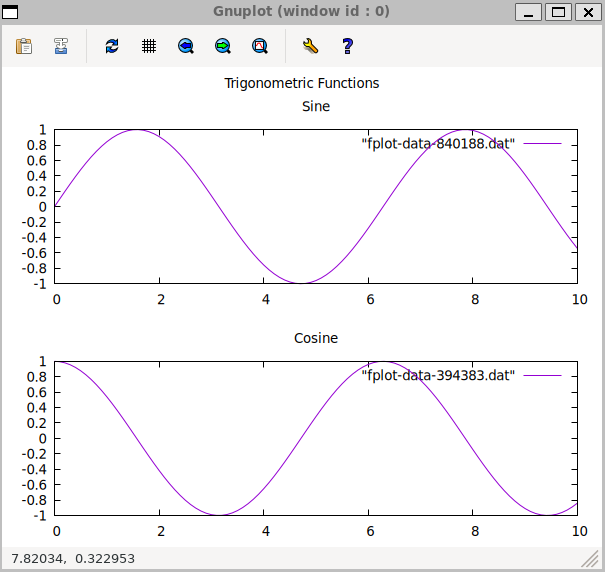
\includegraphics[width=0.6\textwidth]{p6.ex.plot1.png}
		\caption{The resulting plot generated by fplot}
	\end{figure}
	
	\noindent\rule{\textwidth}{0.4pt}
	
	\subsection{Labels, Arrows, and Objects}
	
	You can add arbitrary annotations to your plot using the \texttt{:labels}, \texttt{:arrows}, and \texttt{:objects} options.
	
	\begin{itemize}
		\item \texttt{:labels}: Add text to the plot. Each label is a table \texttt{[text, x, y, options]}.
		\item \texttt{:arrows}: Draw arrows. Each arrow is a table \texttt{[x1, y1, x2, y2, options]}.
		\item \texttt{:objects}: Draw shapes (rectangles, circles, etc.). Each object is a table \texttt{[type, definition]}.
	\end{itemize}
	
	\subsubsection*{Example: Annotating a Peak}
	
	\paragraph{Fennel}
	
	\begin{fennelcode}
(fplot.plot
{:options {:title "Annotated Plot"
		:x-range [0 10]
		:y-range [0 12]
		:labels [["Important Peak" 5 10.5 "center"]]
		:arrows [[7 8 5.2 9.8 "head filled"]]
		:objects [["rectangle" "from 4,0 to 6,10 fs transparent solid 0.1 noborder"]]}
	:datasets [{:data [[1 2] [3 7] [5 10] [7 6] [9 3]]
		:style "linespoints"}]})
	\end{fennelcode}
	
	\paragraph{Lua}
	
	\begin{luacode}
fplot.plot({
	options = {
		title = "Annotated Plot",
		["x-range"] = {0, 10},
		["y-range"] = {0, 12},
		labels = {
			{"Important Peak", 5, 10.5, "center"}
		},
		arrows = {
			{7, 8, 5.2, 9.8, "head filled"}
		},
		objects = {
			{"rectangle", "from 4,0 to 6,10 fs transparent solid 0.1 noborder"}
		}
	},
	datasets = {
		{
			data = {{1, 2}, {3, 7}, {5, 10}, {7, 6}, {9, 3}},
			style = "linespoints"
		}
	}
})
	\end{luacode}
	
	\begin{figure}[H]
		\centering
		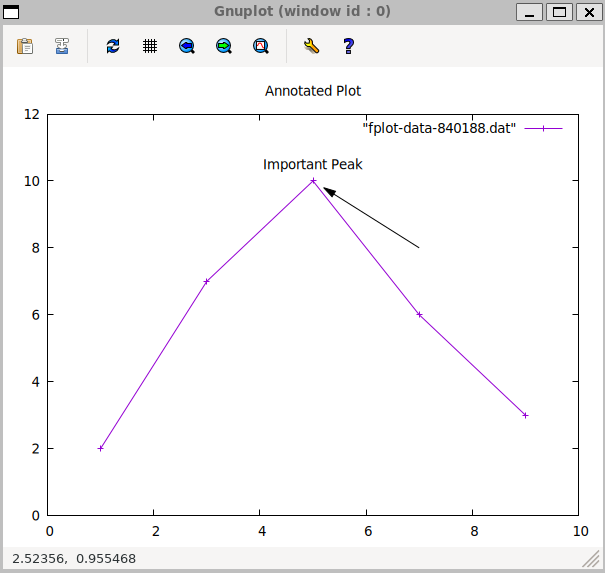
\includegraphics[width=0.6\textwidth]{P6.ex.plot2.png}
		\caption{The resulting plot generated by fplot}
	\end{figure}
	
	\noindent\rule{\textwidth}{0.4pt}
	
	\subsection{Custom Tics}
	
	You can take full control over the axis tic marks using the \texttt{:xtics} and \texttt{:ytics} options. This is useful for categorical data or for highlighting specific points. Provide a list of \texttt{["label", value]} pairs.
	
	\subsubsection*{Example: Labeled Tics}
	
	\paragraph{Fennel}
	
	\begin{fennelcode}
(local fplot (require :fplot))

(fplot.plot
{:options {:title "Quarterly Sales"
		:xtics [["Q1" 1] ["Q2" 2] ["Q3" 3] ["Q4" 4]]
		:ytics [0 10000 20000 30000]
		:y-label "Revenue (\$)"}
	:datasets [{:data [[1 15000] [2 22000] [3 18000] [4 25000]]
		:style "boxes"
		:title "Sales"}]})
	\end{fennelcode}
	
	\paragraph{Lua}
	
	\begin{luacode}
require("fennel").install()
local fplot = require("fplot")

fplot.plot({
	options = {
		title = "Quarterly Sales",
		xtics = {{"Q1", 1}, {"Q2", 2}, {"Q3", 3}, {"Q4", 4}},
		ytics = {0, 10000, 20000, 30000},
		["y-label"] = "Revenue (\$)"
	},
	datasets = {
		{
			data = {{1, 15000}, {2, 22000}, {3, 18000}, {4, 25000}},
			style = "boxes",
			title = "Sales"
		}
	}
})
	\end{luacode}
	
	\begin{figure}[H]
		\centering
		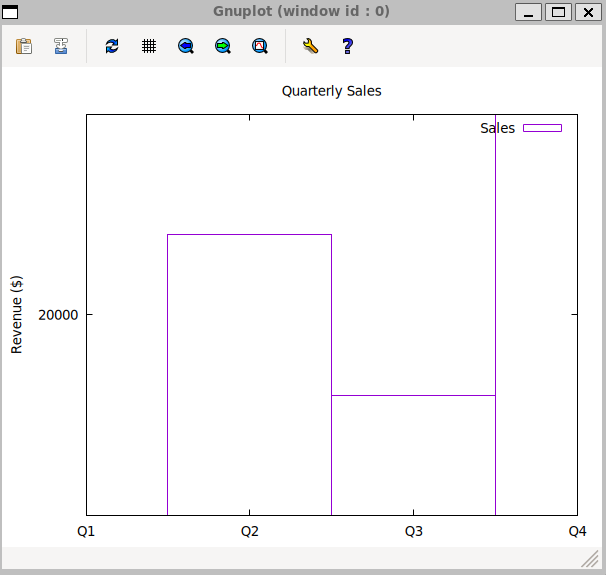
\includegraphics[width=0.6\textwidth]{P6.ex.Plot3.png}
		\caption{The resulting plot generated by fplot}
	\end{figure}
	
	\noindent\rule{\textwidth}{0.4pt}
	
	\subsection{Extra Options (:extra-opts)}
	
	For features that are not directly exposed by \texttt{fplot}, you can use the \texttt{:extra-opts} option to pass raw command strings directly to the Gnuplot script. This provides an escape hatch for accessing the full power of Gnuplot.
	
	\subsubsection*{Example: Setting a Custom Fill Style}
	
	\paragraph{Fennel}
	
	\begin{fennelcode}
(local fplot (require :fplot))

(fplot.plot
{:options {:title "Histogram"
		:extra-opts ["set style fill solid 0.6 border -1"
		"set style histogram clustered gap 2"
		"set style data histograms"]}
	:datasets [{:title "Group A" :data [10 15 12]}
	{:title "Group B" :data [12 11 14]}]})
	\end{fennelcode}
	
	\paragraph{Lua}
	
	\begin{luacode}
require("fennel").install()
local fplot = require("fplot")

fplot.plot({
	options = {
		title = "Histogram",
		["extra-opts"] = {
			"set style fill solid 0.6 border -1",
			"set style histogram clustered gap 2",
			"set style data histograms"
		}
	},
	datasets = {
		{ title = "Group A", data = {10, 15, 12} },
		{ title = "Group B", data = {12, 11, 14} }
	}
})
	\end{luacode}
	
	\begin{figure}[H]
		\centering
		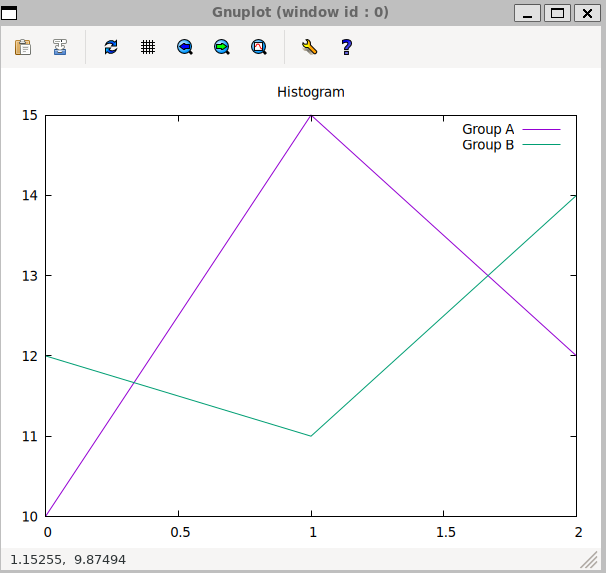
\includegraphics[width=0.6\textwidth]{P6.ex.Plot4.png}
		\caption{The resulting plot generated by fplot}
	\end{figure}
	
	\noindent\rule{\textwidth}{0.4pt}
	
	\newpage
	
	\section{Using Macros and Reusable Components with Fplot}
	
	A key advantage of using a programmatic plotting library like \texttt{fplot} is the ability to create reusable, composable components. This page explains the difference between Gnuplot's native macros and the more flexible approach of using Fennel (or Lua) to manage your plotting.
	
	\subsection{Fennel Macros vs. Lua Functions: A Quick Clarification}
	
	It's important to clarify the term "macro."
	
	\begin{itemize}
		\item \textbf{Fennel}, as a Lisp, has a \textbf{true macro system}. This means Fennel macros are code that writes code, running at \textbf{compile-time} to transform your program before it even becomes Lua. This allows you to create new syntax and fundamentally change how the language works for your specific needs.
		\item \textbf{Lua}, on the other hand, does not have a macro system. When we talk about creating "macros" in a Lua context for \texttt{fplot}, we are using the term informally to describe a powerful \textbf{runtime} pattern: \textbf{reusable functions that generate complex data structures} (like tables for options or datasets). We'll refer to these as "reusable components" or "factory functions" in the Lua examples.
	\end{itemize}
	
	\subsection{Gnuplot's Native Macros}
	
	Gnuplot has a built-in macro system using the \texttt{@} character (e.g., \texttt{plot @my\_macro}). While \texttt{fplot} does not have a feature to directly use these macros in the plot command, you can still \textbf{define} them using the \texttt{:extra-opts} table.
	
	This is useful if you have existing Gnuplot scripts or need to set a simple string substitution.
	
	\begin{fennelcode}
(fplot.plot
{:options {:title "Plotting with a Gnuplot Macro"
		:x-range [-5 5]
		;; Define the macro here
		:extra-opts ["my_func = 'sin(x) / x'"]}
	;; ...
})
	\end{fennelcode}
	
	\subsection{Fennel: The Real Macro System}
	
	The true power of fplot comes from using Fennel itself to create reusable components. Because Fennel has a true macro system, you can create very powerful abstractions. But for most plotting scenerios, simple functions that just return tables are usually more than enough.
	
	\subsubsection*{1. Reusable Data Generators}
	
	You can write functions that generate complex datasets.
	
	\begin{fennelcode}
;; A function for generating sinc data
(fn generate-sinc-data [steps]
(let [data []
step-size (/ 40 steps)]
(for [i (- (/ steps 2)) (/ steps 2)]
(let [x (* i step-size)
row []]
(for [j (- (/ steps 2)) (/ steps 2)]
(let [y (* j step-size)
r (+ (math.sqrt (+ (* x x) (* y y))) 1e-9)
z (/ (math.sin r) r)]
(table.insert row [x y z])))
(table.insert data row)))
data))

;; Use the data generator
(local sinc-data (generate-sinc-data 40))
(fplot.splot {:options {:title "Sinc Function"}
	:datasets [{:data sinc-data :style "pm3d"}]}) 
	\end{fennelcode}
	
	\subsubsection*{2. Reusable Style Templates}
	
	Create functions that return tables with your preferred plot options. This allows you to maintain a consistent style across many different plots.
	
	\begin{fennelcode}
;; A function for a publication-quality plot style
(fn publication-style [title]
{:title title
	:font "Helvetica,14"
	:border true
	:grid true})

;; Use the style template by calling the function
(fplot.plot
{:options (publication-style "My Publication Plot")
	:datasets [...]})
	\end{fennelcode}
	
	\subsubsection*{3. Putting It All Together}
	
	The real magic happens when you combine these components. You can define a base style, a plot-specific style, and then merge them together. The example below is a complete, and runnable script. Feel free to try it!
	
	\paragraph{Fennel}
	
	\begin{fennelcode}
(local fplot (require :fplot))

;; Helper function to recursively clone a table.
(fn table-clone [tbl]
(let [copy {}]
(each [k v (pairs tbl)]
(tset copy k (if (= (type v) "table") (table-clone v) v)))
copy))

;; Helper function to merge tables.
(fn merge-tables [a b]
(let [result (table-clone a)]
(each [k v (pairs b)]
(if (and (= (type v) "table") (= (type (. result k)) "table"))
(tset result k (merge-tables (. result k) v))
(tset result k v)))
result))

;; --- Our Reusable Components ---
(fn generate-line-data [num-points]
(let [data []]
(for [i 1 num-points]
(table.insert data [i (math.random)]))
data))

(fn base-style []
{:font "Arial,12"
	:grid true
	:output-type "pngcairo"
	:size [800 600]})

(fn scatter-plot-style []
{:style "points"
	:pointtype 7
	:color "#3366cc"})

;; --- The Plotting Script ---
(local my-data (generate-line-data 100))

(local plot-specific-opts
{:title "My Composed Plot"
	:x-label "Index"
	:y-label "Random Value"
	:output-file "my-composed-plot.png"})

(local final-options (merge-tables (base-style) plot-specific-opts))
(local final-dataset (merge-tables (scatter-plot-style) {:data my-data}))

(fplot.plot {:options final-options
	:datasets [final-dataset]})

(print "Plot generated at my-new-composed-plot.png")
	\end{fennelcode}
	
	\paragraph{The Lua Equivalent: Reusable Functions}
	
	\begin{luacode}
require("fennel").install()
local fplot = require("fplot")

-- Helper functions
local function table_clone(tbl)
local copy = {}
for k, v in pairs(tbl) do
if type(v) == "table" then
copy[k] = table_clone(v)
else
copy[k] = v
end
end
return copy
end

local function merge_tables(a, b)
local result = table_clone(a)
for k, v in pairs(b) do
if type(v) == "table" and type(result[k]) == "table" then
result[k] = merge_tables(result[k], v)
else
result[k] = v
end
end
return result
end

-- --- Our Reusable Components ---
local function generate_line_data(num_points)
local data = {}
for i = 1, num_points do
table.insert(data, {i, math.random()})
end
return data
end

local function base_style()
return {
	font = "Arial,12",
	grid = true,
	["output-type"] = "pngcairo",
	size = {800, 600}
}
end

local function scatter_plot_style()
return {
	style = "points",
	pointtype = 7,
	color = "#3366cc"
}
end

-- --- The Plotting Script ---
local my_data = generate_line_data(100)

local plot_specific_opts = {
	title = "My Composed Plot",
	["x-label"] = "Index",
	["y-label"] = "Random Value",
	["output-file"] = "my-composed-plot.png"
}

local final_options = merge_tables(base_style(), plot_specific_opts)
local final_dataset = merge_tables(scatter_plot_style(), {data = my_data})

fplot.plot({
	options = final_options,
	datasets = {final_dataset}
})

print("Plot generated at my-composed-plot.png")
	\end{luacode}
	
	\noindent\rule{\textwidth}{0.4pt}
	
	\newpage
	\section{Examples}
	
	This page provides a gallery of examples to showcase the kinds of plots you can create with \texttt{fplot}. Each example includes the code in both Fennel and Lua, along with the resulting plot.
	
	\subsection{1. Line and Point Plot}
	
	A standard plot combining smooth lines and distinct data points.
	
	\subsubsection*{Fennel}
	
	\begin{fennelcode}
(local fplot (require :fplot))

(local data1 [])
(for [i 0 50]
(let [x (* i 0.2)]
(table.insert data1 [x (* (math.exp (* -0.1 x)) (math.cos x))])))

(local data2 [[1 0.5] [3 0.1] [5 -0.2] [7 -0.1] [9 0.05]])

(fplot.plot
{:options {:title "Damped Oscillation with Data Points"
		:x-label "Time"
		:y-label "Amplitude"
		:grid true
		:key {:position "top right"}}
	:datasets [{:title "Model"
		:style "lines"
		:color "blue"
		:data data1}
	{:title "Measurements"
		:style "points"
		:color "red"
		:pointtype 7
		:data data2}]})
	\end{fennelcode}
	
	\subsubsection*{Lua}
	
	\begin{luacode}
require("fennel").install()
local fplot = require("fplot")

local data1 = {}
for i = 0, 50 do
local x = i * 0.2
table.insert(data1, {x, math.exp(-0.1 * x) * math.cos(x)})
end

local data2 = {{1, 0.5}, {3, 0.1}, {5, -0.2}, {7, -0.1}, {9, 0.05}}

fplot.plot({
	options = {
		title = "Damped Oscillation with Data Points",
		x_label = "Time",
		y_label = "Amplitude",
		grid = true,
		key = {position = "top right"}
	},
	datasets = {
		{
			title = "Model",
			style = "lines",
			color = "blue",
			data = data1
		},
		{
			title = "Measurements",
			style = "points",
			color = "red",
			pointtype = 7,
			data = data2
		}
	}
})
	\end{luacode}
	
	\begin{figure}[H]
		\centering
		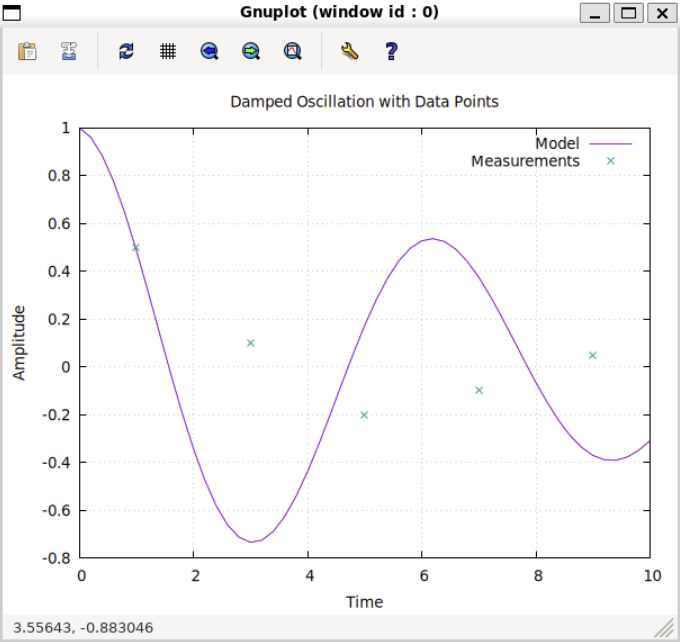
\includegraphics[width=0.6\textwidth]{P8.ex.Plot1.png}
		\caption{The resulting plot generated by fplot}
	\end{figure}
	
	\noindent\rule{\textwidth}{0.4pt}
	
	\subsection{2. Bar Chart / Histogram}
	
	Creating a bar chart using the \texttt{boxes} style, which is great for categorical data.
	
	\subsubsection*{Fennel}
	
	\begin{fennelcode}
(local fplot (require :fplot))

(fplot.plot
{:options {:title "Annual Production by Factory"
		:y-label "Units Produced"
		:x-range [0.5 4.5]
		:y-range [0 50000]
		:xtics [["North" 1] ["South" 2] ["East" 3] ["West" 4]]
		:extra-opts ["set style fill solid 0.8"]}
	:datasets [{:title "Production"
		:style "boxes"
		:data [[1 42000] [2 35000] [3 48000] [4 29000]]}]})
	\end{fennelcode}
	
	\subsubsection*{Lua}
	
	\begin{luacode}
require("fennel").install()
local fplot = require("fplot")

fplot.plot({
	options = {
		title = "Annual Production by Factory",
		y_label = "Units Produced",
		x_range = {0.5, 4.5},
		y_range = {0, 50000},
		xtics = {{"North", 1}, {"South", 2}, {"East", 3}, {"West", 4}},
		extra_opts = {"set style fill solid 0.8"}
	},
	datasets = {
		{
			title = "Production",
			style = "boxes",
			data = {{1, 42000}, {2, 35000}, {3, 48000}, {4, 29000}}
		}
	}
})
	\end{luacode}
	
	\begin{figure}[H]
		\centering
		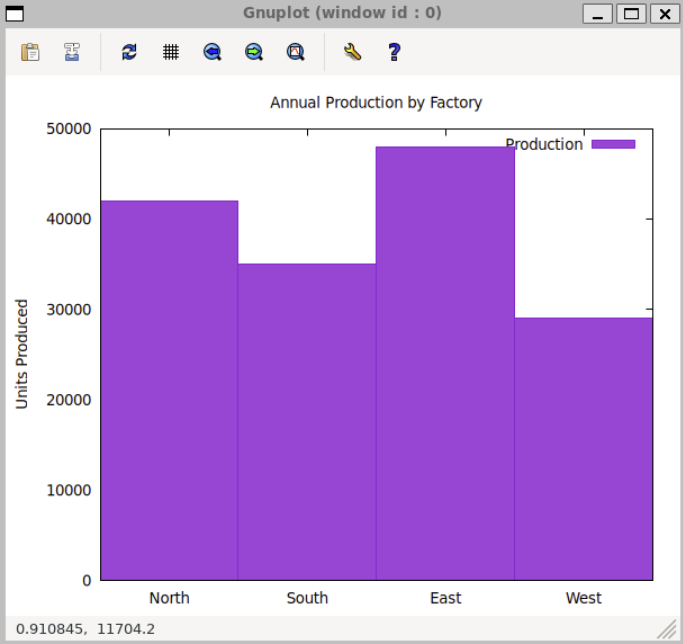
\includegraphics[width=0.6\textwidth]{P8.ex.Plot2.png}
		\caption{The resulting plot generated by fplot}
	\end{figure}
	
	\noindent\rule{\textwidth}{0.4pt}
	
	\subsection{3. 3D Surface Plot}
	
	Using \texttt{fplot.splot} to visualize three-dimensional data.
	
	\subsubsection*{Fennel}
	
	\begin{fennelcode}
(local fplot (require :fplot))

(local data [])
(for [i -20 20]
(let [x (* i 0.5)
row []]
(for [j -20 20]
(let [y (* j 0.5)
r (+ (math.sqrt (+ (* x x) (* y y))) 1e-6)
z (/ (math.sin r) r)]
(table.insert row [x y z])))
(table.insert data row)))

(fplot.splot
{:options {:title "Sinc Function"
		:z-label "z"
		:palette "viridis"}
	:datasets [{:data data
		:style "pm3d"
		:title ""}]})
	\end{fennelcode}
	
	\subsubsection*{Lua}
	
	\begin{luacode}
require("fennel").install()
local fplot = require("fplot")

local data = {}
for i = -20, 20 do
local x = i * 0.5
local row = {}
for j = -20, 20 do
local y = j * 0.5
local r = math.sqrt(x*x + y*y) + 1e-6
local z = math.sin(r) / r
table.insert(row, {x, y, z})
end
table.insert(data, row)
end

fplot.splot({
	options = {
		title = "Sinc Function",
		z_label = "z",
		palette = "viridis"
	},
	datasets = {
		{
			data = data,
			style = "pm3d",
			title = ""
		}
	}
})
	\end{luacode}
	
	\begin{figure}[H]
		\centering
		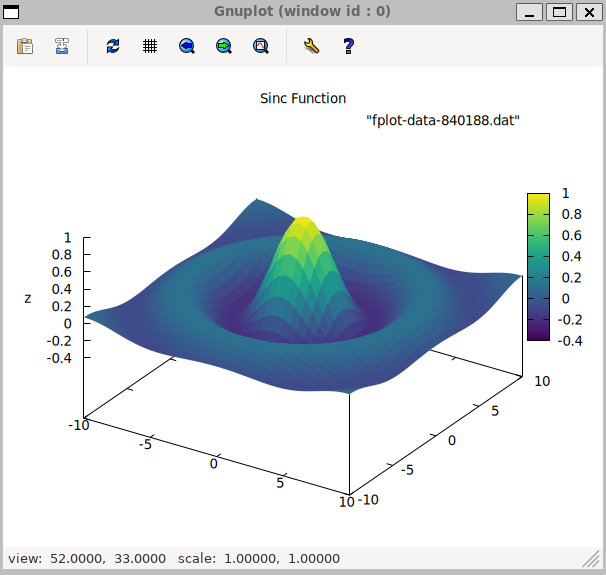
\includegraphics[width=0.6\textwidth]{P1.P8.ex.Plot1.Plot3.png}
		\caption{The resulting plot generated by fplot}
	\end{figure}
	
	\noindent\rule{\textwidth}{0.4pt}
	
	\subsection{4. Logarithmic Scale Plot}
	
	Useful for visualizing data that spans several orders of magnitude.
	
	\subsubsection*{Fennel}
	
	\begin{fennelcode}
(local fplot (require :fplot))

(local data [])
(for [x 1 100]
(table.insert data [x (* 1000 (math.exp (* -0.1 x)))]))

(fplot.plot
{:options {:title "Exponential Decay"
		:x-label "Time"
		:y-label "Value"
		:log-scale "y"
		:grid true}
	:datasets [{:title "Decay"
		:style "lines"
		:data data}]})
	\end{fennelcode}
	
	\subsubsection*{Lua}
	
	\begin{luacode}
require("fennel").install()
local fplot = require("fplot")

local data = {}
for x = 1, 100 do
table.insert(data, {x, 1000 * math.exp(-0.1 * x)})
end

fplot.plot({
	options = {
		title = "Exponential Decay",
		x_label = "Time",
		y_label = "Value",
		log_scale = "y",
		grid = true
	},
	datasets = {
		{
			title = "Decay",
			style = "lines",
			data = data
		}
	}
})
	\end{luacode}
	
	\begin{figure}[H]
		\centering
		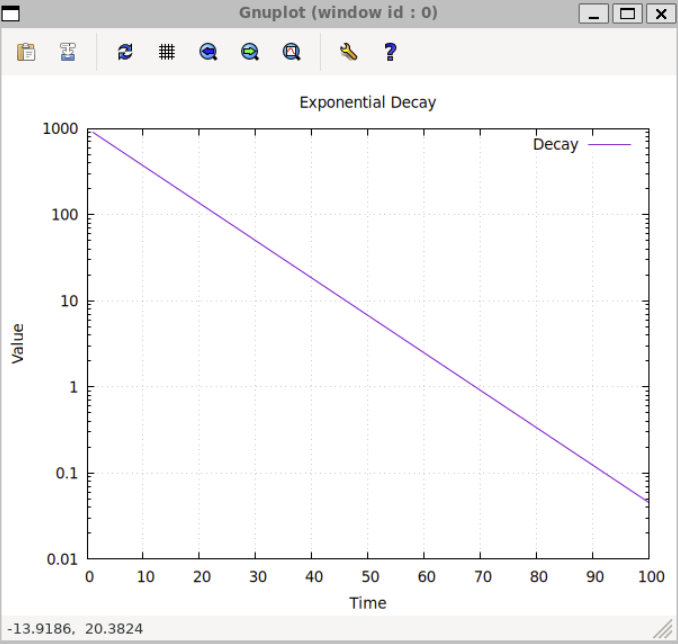
\includegraphics[width=0.6\textwidth]{P8.ex.Plot4.png}
		\caption{The resulting plot generated by fplot}
	\end{figure}
	
	\noindent\rule{\textwidth}{0.4pt}
	
	\newpage
	
	\section{Biotech Applications}
	
	This page demonstrates how to generate plots commonly used in Biotech.
	
	\subsection{1. Volcano Plot for Gene Expression}
	
	Volcano plots are used to visualize differential gene expression results of RNA-Seq and/or microarray experiments. They plot statistical significance (-log10 p-value) against magnitude of change (log2 fold change).
	
	This example shows how to create a volcano plot, highlighting significantly up- and down-regulated genes.
	
	\subsubsection*{Fennel}
	
	\begin{fennelcode}
(local fplot (require :fplot))

;; --- Mock Data Generation ---
(math.randomseed 42)
(local up-regulated [])
(local down-regulated [])
(local non-significant [])

(for [_ 1 500]
(let [log2fc (- -4 (* (math.random) 4)) ; range [-8, -4]
p-value (* (math.random) 1e-6)]
(table.insert down-regulated [log2fc (* -1 (math.log10 p-value))])))

(for [_ 1 500]
(let [log2fc (+ 4 (* (math.random) 4)) ; range [4, 8]
p-value (* (math.random) 1e-6)]
(table.insert up-regulated [log2fc (* -1 (math.log10 p-value))])))

(for [_ 1 9000]
(let [log2fc (* (- (math.random) 0.5) 8) ; range [-4, 4]
p-value (math.random)]
(table.insert non-significant [log2fc (* -1 (math.log10 p-value))])))


;; --- Plotting ---
(fplot.plot
{:options {:title "Volcano Plot of Differential Gene Expression"
		:x-label "log2(Fold Change)"
		:y-label "-log10(p-value)"
		:grid true
		:key {:enabled false}}
	:datasets [{:style "points" :pointtype 7 :color "#cccccc" :data non-significant}
	{:style "points" :pointtype 7 :color "#ff4136" :data up-regulated}
	{:style "points" :pointtype 7 :color "#0074d9" :data down-regulated}]})
\end{fennelcode}
	
	\subsubsection*{Lua}
	
	\begin{luacode}
require("fennel").install()
local fplot = require("fplot")

-- --- Mock Data Generation ---
math.randomseed(42)
local up_regulated = {}
local down_regulated = {}
local non_significant = {}

for _ = 1, 500 do
local log2fc = -4 - math.random() * 4
local p_value = math.random() * 1e-6
table.insert(down_regulated, {log2fc, -math.log10(p_value)})
end

for _ = 1, 500 do
local log2fc = 4 + math.random() * 4
local p_value = math.random() * 1e-6
table.insert(up_regulated, {log2fc, -math.log10(p_value)})
end

for _ = 1, 9000 do
local log2fc = (math.random() - 0.5) * 8
local p_value = math.random()
table.insert(non_significant, {log2fc, -math.log10(p_value)})
end

-- --- Plotting ---
fplot.plot({
	options = {
		title = "Volcano Plot of Differential Gene Expression",
		x_label = "log2(Fold Change)",
		y_label = "-log10(p-value)",
		grid = true,
		key = {enabled = false}
	},
	datasets = {
		{style = "points", pointtype = 7, color = "#cccccc", data = non_significant},
		{style = "points", pointtype = 7, color = "#ff4136", data = up_regulated},
		{style = "points", pointtype = 7, color = "#0074d9", data = down_regulated}
	}
})
	\end{luacode}
	
	\begin{figure}[H]
		\centering
		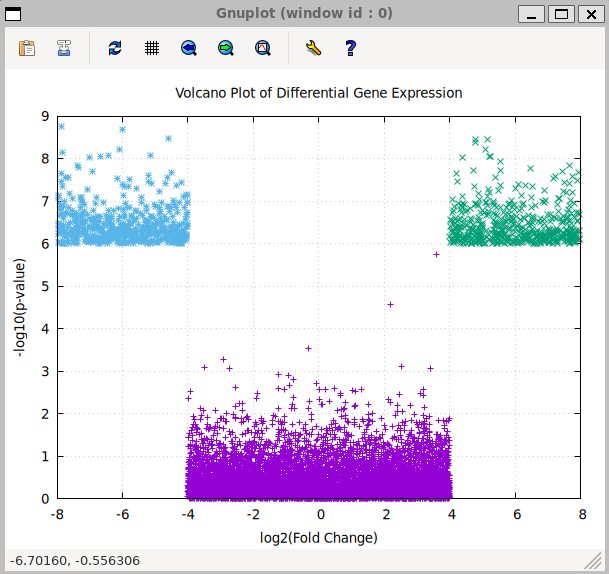
\includegraphics[width=0.6\textwidth]{P9.ex.Plot1.png}
		\caption{The resulting plot generated by fplot}
	\end{figure}
	
	\noindent\rule{\textwidth}{0.4pt}
	
	\subsection{2. Protein Thermal Melt Curve}
	
	A thermal melt curve from a Differential Scanning Fluorimetry (DSF) experiment is used to assess protein stability. This plot shows fluorescence vs. temperature, and the inflection point of the curve is the melting temperature (Tm). This example plots two curves, representing a protein with and without a stabilizing ligand.
	
	\subsubsection*{Fennel}
	
	\begin{fennelcode}
(local fplot (require :fplot))

;; --- Mock Data Generation ---
(fn sigmoid [x x0 k]
(/ 1 (+ 1 (math.exp (- (* k (- x x0)))))))

(local protein-only [])
(local with-ligand [])
(for [temp 25 95 1]
(let [base-fluor (* (math.random) 0.1)
tm1 55
tm2 65]
(table.insert protein-only [temp (+ 10 base-fluor (* 80 (sigmoid temp tm1 0.5)))])
(table.insert with-ligand [temp (+ 10 base-fluor (* 80 (sigmoid temp tm2 0.5)))])))

;; --- Plotting ---
(fplot.plot
{:options {:title "Protein Thermal Shift Assay"
		:x-label "Temperature (°C)"
		:y-label "Relative Fluorescence Units (RFU)"
		:key {:position "bottom right"}}
	:datasets [{:title "Apo Protein"
		:style "lines"
		:color "black"
		:data protein-only}
	{:title "Protein + Ligand"
		:style "lines"
		:color "blue"
		:data with-ligand}]})
	\end{fennelcode}
	
	\subsubsection*{Lua}
	
	\begin{luacode}
require("fennel").install()
local fplot = require("fplot")

-- --- Mock Data Generation ---
local function sigmoid(x, x0, k)
return 1 / (1 + math.exp(-k * (x - x0)))
end

local protein_only = {}
local with_ligand = {}
for temp = 25, 95, 1 do
local base_fluor = math.random() * 0.1
local tm1 = 55
local tm2 = 65
table.insert(protein_only, {temp, 10 + base_fluor + 80 * sigmoid(temp, tm1, 0.5)})
table.insert(with_ligand, {temp, 10 + base_fluor + 80 * sigmoid(temp, tm2, 0.5)})
end

-- --- Plotting ---
fplot.plot({
	options = {
		title = "Protein Thermal Shift Assay",
		x_label = "Temperature (°C)",
		y_label = "Relative Fluorescence Units (RFU)",
		key = {position = "bottom right"}
	},
	datasets = {
		{
			title = "Apo Protein",
			style = "lines",
			color = "black",
			data = protein_only
		},
		{
			title = "Protein + Ligand",
			style = "lines",
			color = "blue",
			data = with_ligand
		}
	}
})
	\end{luacode}
	
	\begin{figure}[H]
		\centering
		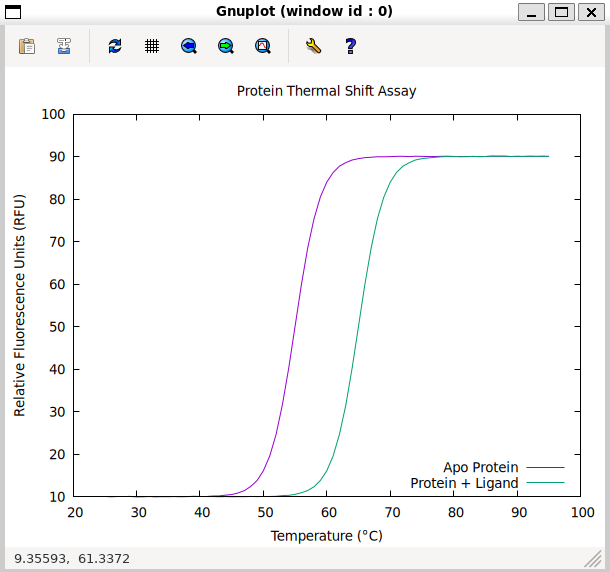
\includegraphics[width=0.6\textwidth]{P9.ex.Plot2.png}
		\caption{The resulting plot generated by fplot}
	\end{figure}
	
	\noindent\rule{\textwidth}{0.4pt}
	
	\newpage
	
	\section{Troubleshooting Guide}
	
	This guide provides solutions to common problems you might encounter when using \texttt{fplot} in different environments.
	
	\subsection{General Issues}
	
	\subsubsection*{Problem: \texttt{gnuplot} not found or command fails.}
	
	When you run an \texttt{fplot} script, and you see an error like \texttt{sh: gnuplot: command not found} or a non-zero exit code.
	
	\textbf{Solution:}
	
	\begin{enumerate}
		\item \textbf{Verify \texttt{gnuplot} Installation:} Make sure \texttt{gnuplot} is installed on your system. See the \href{https://www.google.com/search?q=https://github.com/your-username/fplot/wiki/Installation}{Installation} guide.
		\item \textbf{Check System \texttt{PATH}:} The \texttt{gnuplot} executable must be in your system's \texttt{PATH}. You can check this by opening a terminal and typing \texttt{gnuplot --version}. If it's not found, you need to add its location to your \texttt{PATH} environment variable.
		\item \textbf{Hardcode the Path:} As a last resort, you can edit your local \texttt{fplot.fnl} (or \texttt{fplot.lua}) file and change the \texttt{gnuplot-executable} variable to the full, absolute path of the \texttt{gnuplot} executable on your system.
	\end{enumerate}
	
	\subsubsection*{Problem: The plot window appears and immediately closes.}
	
	\textbf{Solution:}
	
	This typically happens when gnuplot is not run in "persistent" mode. fplot automatically handles this by adding the -p flag or a pause mouse close command when it's not saving to a file. If you are running gnuplot scripts manually, make sure to use the -p flag: \texttt{gnuplot -p your\_script.gp}.
	
	\subsection{MSYS2 (on Windows)}
	
	The MSYS2 environment can be tricky because of how it handles file paths.
	
	\subsubsection*{Problem: \texttt{fplot} fails with errors like "Can't open script file" or "Cannot find data file".}
	
	This is the most common issue on MSYS2 and is caused by \textbf{path mangling}. MSYS2 automatically converts POSIX-style paths (e.g., \texttt{/c/Users/Me}) to Windows-style paths (\texttt{C:\textbackslash Users\textbackslash Me}) when calling native Windows programs like \texttt{gnuplot}. This can corrupt the paths to the temporary script and data files that \texttt{fplot} creates.
	
	\textbf{Solution 1: Disable Path Mangling (Recommended)}
	
	You can tell MSYS2 not to convert paths by setting an environment variable before running your script.
	
	\begin{bashcode}
# In your MSYS2 terminal
export MSYS2_ARG_CONV_EXCL="*"
fennel your_plot_script.fnl
	\end{bashcode}
	
	To make this permanent, add \texttt{export MSYS2\_ARG\_CONV\_EXCL="*"} to your \texttt{\textasciitilde/.bashrc} or \texttt{\textasciitilde/.bash\_profile} file in your MSYS2 home directory.
	
	\textbf{Solution 2: Use the MinGW \texttt{gnuplot} Package}
	
	Within your MSYS2 environment, it's best to use the \texttt{gnuplot} package from the MinGW repositories, as it's a native Windows build that integrates well with the environment. You can install it using \texttt{pacman}:
	
	\begin{bashcode}
pacman -S mingw-w64-x86_64-gnuplot
	\end{bashcode}
	
	This version is generally more reliable for GUI applications than a purely POSIX-emulated build. However, even with this version, the path mangling described in Solution 1 is often still a problem, so disabling it is the most robust fix.
	
	\subsection{WSL2 (Windows Subsystem for Linux)}
	
	WSL2 runs a full Linux kernel. On modern Windows 10 and 11, the \textbf{WSLg} feature provides built-in support for Linux GUI applications, so they should work out of the box.
	
	\textbf{Problem:} The script runs, but no plot window appears. You might see an error like "cannot open display" or "Gnuplot terminal type set to 'unknown'".
	
	\textbf{Solution for Modern Windows (with WSLg):}
	
	\begin{enumerate}
		\item \textbf{Ensure WSL is Up-to-Date:} Open a Windows PowerShell or Command Prompt and run \texttt{wsl --update}. This will ensure you have the latest version with WSLg.
		\item \textbf{Install a GUI-enabled \texttt{gnuplot}:} Your Linux distribution needs a version of \texttt{gnuplot} that can create a graphical window.
		\begin{bashcode}
# On Debian/Ubuntu
sudo apt-get update
sudo apt-get install gnuplot-x11
		\end{bashcode}
		This should be all you need. When you run your \texttt{fplot} script from WSL2, the plot window should appear on your Windows desktop automatically(appearance is slow).
	\end{enumerate}
	
	\textbf{Solution for Older Windows Versions (without WSLg):}
	
	If you are on an older build of Windows that doesn't support WSLg, you will need to manually install an X server on Windows.
	
	\begin{enumerate}
		\item \textbf{Install an X Server on Windows:} Download and install a free X server like \href{https://sourceforge.net/projects/vcxsrv/}{VcXsrv} on your Windows machine.
		\item \textbf{Launch the X Server:} Launch VcXsrv and choose "Multiple windows", "Display number -1", and on the final page, check "Disable access control".
		\item \textbf{Configure the \texttt{DISPLAY} Variable in WSL2:} Your Linux environment needs to know where the display is. Add the following line to your \texttt{\textasciitilde/.bashrc} file in your WSL2 home directory:
		\begin{bashcode}
export DISPLAY=$(cat /etc/resolv.conf | grep nameserver | awk '{print $2; exit;}'):0.0
		\end{bashcode}
		\item \textbf{Reload Your Shell:} Close and reopen your WSL2 terminal, or run \texttt{source \textasciitilde/.bashrc}. After this, GUI applications from WSL2 should appear on your desktop.
	\end{enumerate}
	
	\subsection{Native Linux / macOS}
	
	\texttt{fplot} is most at home on these systems and issues are rare.
	
	\subsubsection*{Problem: \texttt{fplot} complains about a missing terminal type (e.g., "Terminal type set to 'unknown'").}
	
	\textbf{Solution:}
	
	Your gnuplot installation may be missing support for interactive terminals. When you installed gnuplot, you may have gotten a "core" or "nogui" version. Re-install it and ensure you get a version with qt or x11 support.
	
	\begin{itemize}
		\item \textbf{Debian/Ubuntu:} \texttt{sudo apt-get install gnuplot-x11} or \texttt{sudo apt-get install gnuplot-qt}
		\item \textbf{Arch Linux:} The default \texttt{gnuplot} package should be sufficient.
		\item \textbf{macOS (Homebrew):} \texttt{brew install gnuplot} should install a version with the \texttt{qt} terminal.
	\end{itemize}
	
	You can check which terminals your \texttt{gnuplot} supports by running \texttt{gnuplot -e "show terminal"}.
	
	\subsection{A Note on Gnuplot Terminals (GUI Backends)}
	
	\subsubsection*{Problem: A plot window appears, but it's buggy, slow, or doesn't appear at all, even though \texttt{gnuplot} is installed correctly.}
	
	\textbf{Solution:}
	
	gnuplot uses different internal engines, called "terminals," to draw its interactive plot windows. The most common ones are wxt (the default on many systems), qt, and x11. Sometimes, the default terminal may have issues with your specific desktop environment or system configuration, especially in complex setups like MSYS2.
	
	If you suspect this is the issue, you can force \texttt{fplot} to use a different terminal by setting the \texttt{:output-type} option in your plot configuration.
	
	\textbf{Example (forcing the \texttt{qt} terminal):}
	
	\begin{fennelcode}
(fplot.plot
{:options {:title "My Plot"
		:output-type "qt"} ; <-- Force the qt terminal
	:datasets [;...
	]})
	\end{fennelcode}
	
	This is a powerful troubleshooting step. If the default \texttt{wxt} terminal fails, try \texttt{qt}. If \texttt{qt} fails, try \texttt{x11} (on Linux). Make sure you have the necessary support libraries installed for the terminal you want to use (e.g., the \texttt{gnuplot-qt} package on Debian/Ubuntu for the \texttt{qt} terminal).
	
	\printbibliography
\end{document}